\section{Introduction}
\dropcap{R}obots have long been used in industrial tasks requiring precision and strength, such as assembly and manufacturing~\citep{todd1996fundamentals}. However, societal challenges now call for robots designed for human-centered environments like homes and public spaces~\citep{nahavandi2019industry, chibani2013ubiquitous, royakkers2015literature}. To operate safely in dynamic, unpredictable settings—and in line with Asimov’s First Law to avoid harming humans~\citep{asimov1941three, villani2018survey}—robots should incorporate inherent physical compliance. Modern systems use advanced controls like safety filters, compliant control, real-time collision detection, and predefined safety zones~\citep{zhao2024potential}, relying on sophisticated sensors and algorithms to preempt hazards~\citep{fragapane2021planning}. Collaborative robots (cobots) are designed with decoupled actuators, reduced inertia, and compliant controllers for safer human interaction, yet their rigid components can still pose risks~\citep{haddadin2009requirements}. Although collision detection can mitigate danger by slowing or stopping robots near humans~\citep{haddadin2013towards}, it does not completely eliminate injury risk.

Soft robotics offers a transformative approach by embedding safety directly into a robot’s materials and structure, reducing reliance on complex computational algorithms~\citep{rus2015design, laschi2016soft}. This inherent compliance enables safe human interaction and operation in sensitive settings such as personal assistance, caregiving, and handling delicate items~\citep{abidi2017intrinsic, pasquier2025study}. However, soft robot development is inherently complex, requiring the seamless integration of materials, geometry, actuation, sensing, compliant continuum dynamics, perception, and control systems. It is notably difficult to predict how morphological changes affect closed-loop motion, as the design space is much larger than for rigid robots, and the capabilities of the autonomy stack and control are inherently limited by the body. For some morphologies with very complex deformations, designing effective proprioception and control systems is even intractable. Consequently, we observe that traditional sequential design processes~\citep{van2020delft}—which move from conceptual design through mechatronic design to the development of autonomy and control systems—struggle with this complexity, leading to robots that exhibit imprecise, oscillatory motions, limited payload capacity, and inadequate force output~\citep{iida2011soft, cianchetti2013stiff, mazzolai2022roadmap, majidi2014soft, hawkes2017soft}.

\paragraph*{Related Work and Limitations}
Co-design strategies have proven effective in addressing multi-objective problems and accommodating the compositional, hierarchical nature of complex systems~\citep{zardini2023co}. 
In this perspective, we review recent studies that have introduced algorithms for simultaneous optimization of soft robot morphology and control systems~\citep{van2018spatial, spielberg2019learning, chen2020design, bhatia2021evolution, spielberg2021co, wang2023preco, medvet2021biodiversity, wang2022curriculum, junge2022leveraging, legrand2023reconfigurable, wang2024diffusebot, navez2024contributions}. 
However, we identify several shortcomings that limit their broader application. 
First, computationally expensive optimization cycles hinder exploration of the full design space~\citep{chen2020design}, due to high-dimensional discretizations~~\citep{spielberg2019learning, medvet2021biodiversity, medvet2022impact, wang2022curriculum, legrand2023reconfigurable, wang2023softzoo, wang2023preco, wang2024diffusebot}, inefficient algorithms (e.g., evolutionary ones)~\citep{chen2020design, rieffel2014growing, hiller2012automatic, bhatia2021evolution, medvet2021biodiversity, medvet2022impact}, costly \gls{RL}-based control training~~\citep{bhatia2021evolution, wang2022curriculum, wang2023softzoo, wang2023preco}, and reliance on intensive simulations for fitness evaluation~~\citep{spielberg2019learning, medvet2021biodiversity, medvet2022impact, wang2022curriculum, legrand2023reconfigurable, wang2023softzoo, wang2023preco, wang2024diffusebot}.
Second, a narrow focus on easily computable evaluation metrics (e.g., locomotion speed~\citep{wang2024diffusebot}, workspace~\citep{guan2023trimmed}) often neglects other vital design values such as manufacturability~\citep{kim2025generative}, safety, cost, ecological impact, usability, and regulatory requirements~\citep{junge2022leveraging}. 
Third, the actual realization of the design is rarely~\citep{junge2022leveraging} factored into the co-design optimization process, which limits the incorporation of insights gained from fabrication, prototyping, and lab/field testing. Similarly, the uncertainty associated with simulation-derived evaluation metrics is seldom considered~\citep{chen2020design}, leading to designs that perform well in simulations but underperform in real-world scenarios.
% 
Finally, current co-design methods generally fail to incorporate diverse stakeholder input or account for (all) end-user requirements.

We recognize that parallel yet disconnected efforts exist to address these challenges. For instance, efficient category theory–based algorithms have recently been developed for the co‑design of self‑driving vehicles, considering diverse design values such as cost, compute requirements, vehicle mass, and power~\citep{zardini2021co,zardini2022task,milojevic2025codei}. In \gls{ML}, there is a strong emphasis on generative models for design generation~\citep{vahdat2022lion}, with recent applications in soft robot co‑design~\citep{song2024morphvae, wang2024diffusebot}, enabling optimization in a reduced‑order space while recovering the full design description. Furthermore, literature in ML and soft robotics explores how to learn reduced‑order dynamic models for efficient model‑based controller derivation~\citep{hewing2020learning, alora2023data, della2023model, stolzle2024input, alkayas2025soft} as an alternative to sample‑inefficient \gls{RL}. Additionally, concepts from nonlinear systems and robotics—such as observability~\citep{griffith1971observability}, controllability~\citep{zheng2019controllability}, and safety~\citep{haddadin2013towards, iso2016collaborative}—offer computationally inexpensive metrics to assess design fitness. Finally, a robust body of work in Bayesian optimization~\citep{hernandez2014predictive, garnett2023bayesian}, \gls{RL}~\citep{sutton1998reinforcement}, and co‑design~\citep{huang2025composable, furter2025composable} has explored incorporating uncertainty in evaluation metrics during optimization and using exploration (i.e., realization) to reduce that uncertainty. The goal of this perspective is to synthesize these related yet isolated research directions into a holistic co‑design framework that addresses the shortcomings of existing approaches.

\paragraph*{Proposed Framework}
This perspective outlines a holistic co-design framework that integrates design components, stakeholder values, design processes, and optimization strategies, addressing key limitations of prior soft robotic co-design approaches through five core advances.
First, the framework broadens the range of considered objectives and constraints to include safety, fabrication and operational costs, environmental impact, and regulatory compliance.
Second, we introduce enhancements to computational co-design, boosting computational efficiency and allowing for global optimization over the design space.
Specifically, this is achieved by (i) sampling from reduced-order design spaces decoded into full morphologies~\citep{wang2024diffusebot}; (ii) co-optimizing reduced-order dynamical models, both physics-based~\citep{armanini2023soft} and learned~\citep{liu2024physics, stolzle2024input, valadas2025learning, alkayas2025soft, navez2025modeling}, to capture task-relevant deformations with minimal complexity; (iii) using fast-to-compute surrogate metrics (e.g., controllability or observability) to guide the optimizer away from poor designs early in the process; and (iv) replacing costly \gls{RL} training with efficient model-based control methodologies grounded in the same reduced-order models~\citep{della2023model,stolzle2024input}.
Third, the framework incorporates purposeful physical prototyping to reduce uncertainty in computational evaluations.
By treating co-design probabilistically, it accounts for uncertainties, such as the sim-to-real gap~\citep{dubied2022sim}, and uses high-fidelity simulation and prototyping across varying \glspl{TRL}~\citep{NASA_TRL} to refine evaluation metric estimates.
This enables formal trade-offs between computational ``refinement'' and physical ``realization'', taming the sim-to-real gap discrepancies in performances during the development cycle.
Fourth, the integration of structured stakeholder engagement ensures that diverse values and requirements are reflected throughout the design process.
Finally, the framework supports reproducibility~\citep{baines2024need} by maintaining an auditable design trail, which is critical for the deployment of soft robots in real-world contexts.

\begin{figure}[tb]
    \centering
    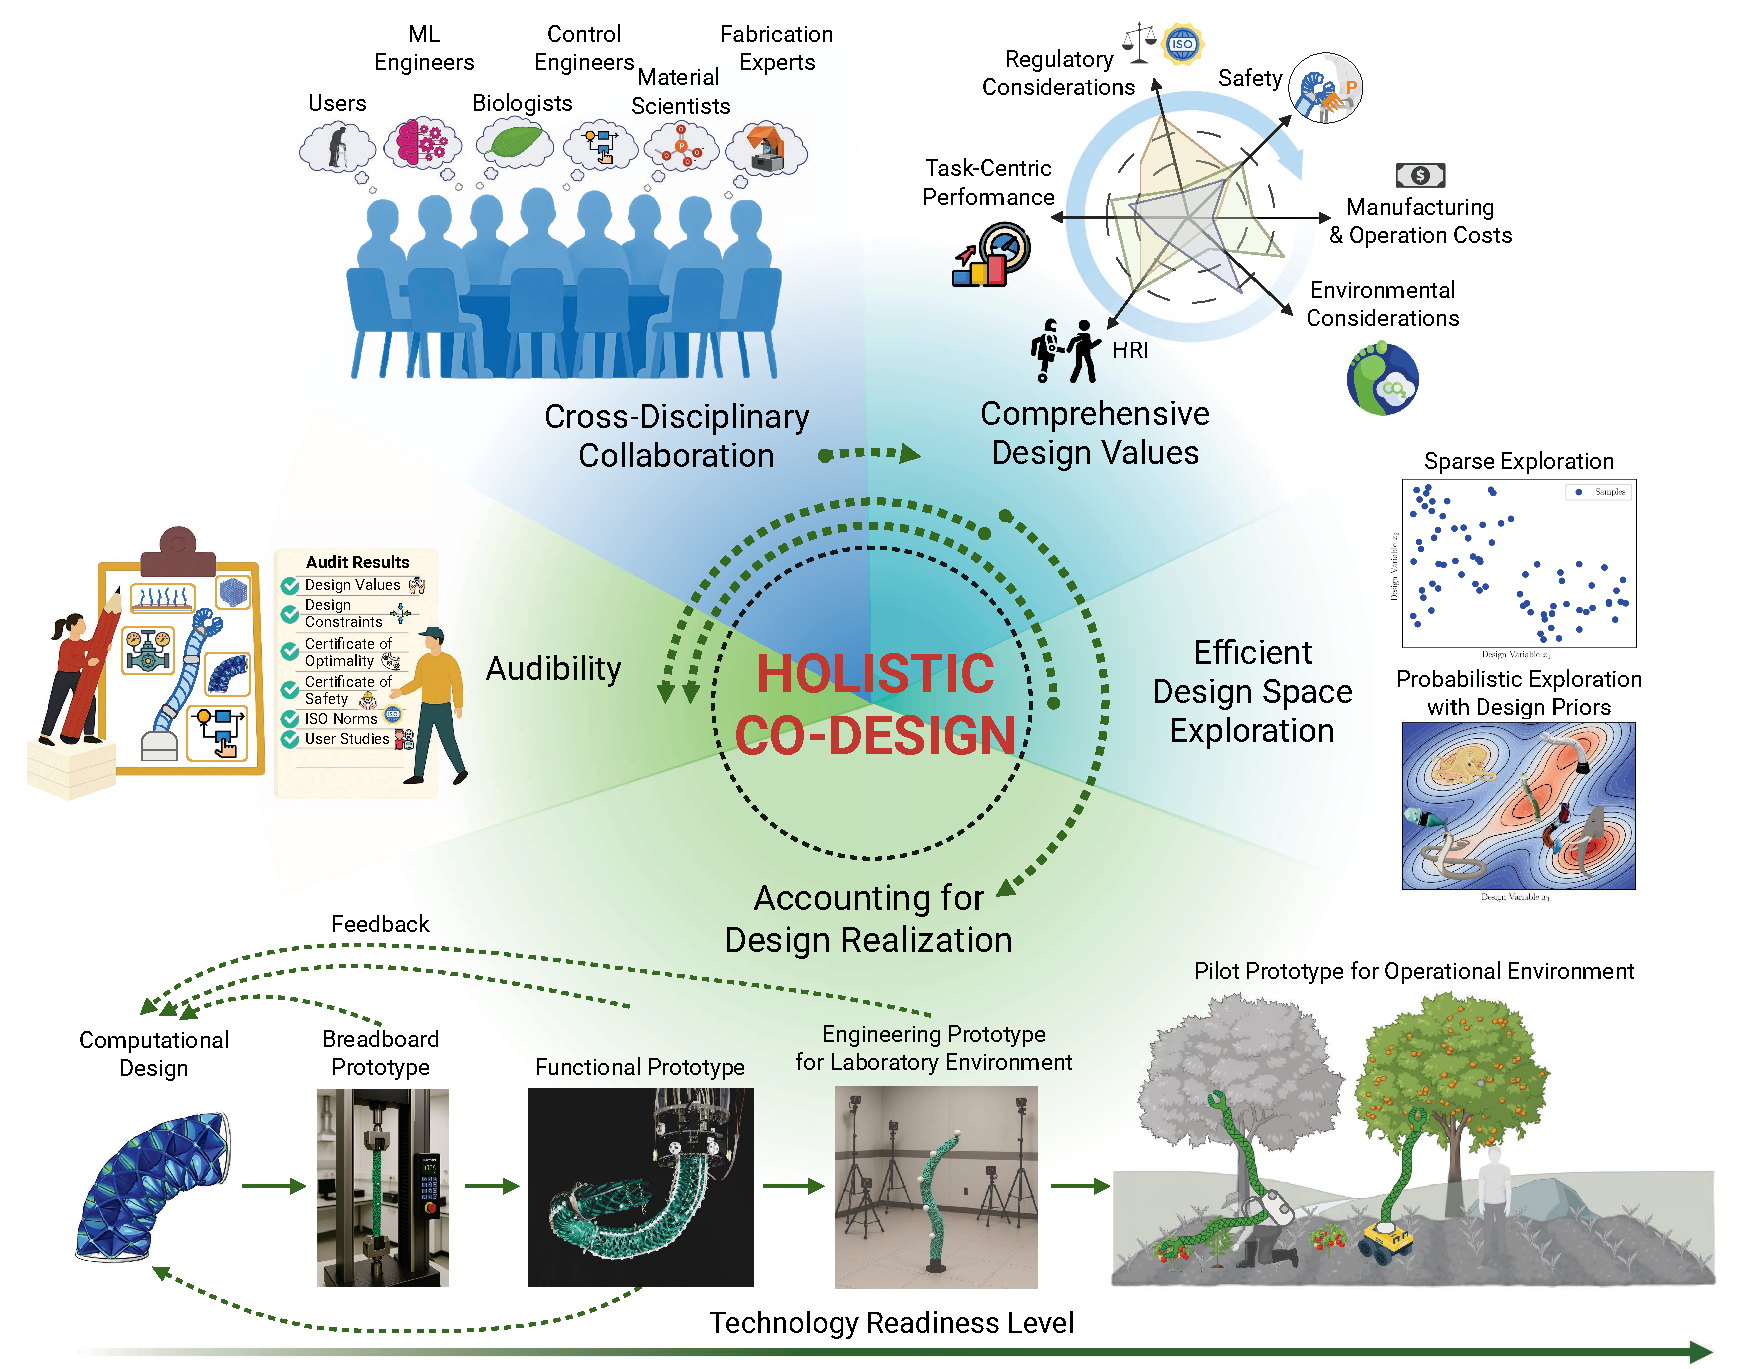
\includegraphics[width=\textwidth]{appendix-holistic-codesign/figures/holistic_codesign_overview_layered_optimized.pdf}
    \caption{
    \textbf{Holistic Co-Design of Soft Robots.}
    The five pillars of holistic co‑design are (1) Incorporating comprehensive design requirements and values directly into multi‑objective optimization; (2) Efficiently exploring the full design space by melding design priors (e.g., biological inspirations, existing solutions) with computationally efficient co‑design routines; (3) Explicitly accounting for design realization (e.g., prototyping and testing) via a probabilistic treatment of evaluation metrics and by formalizing the refinement‑vs‑realization trade‑off—enabling targeted prototyping to reduce metric uncertainty and narrow the sim‑to‑real gap; (4) Fostering cross‑disciplinary collaboration and involving all relevant stakeholders in defining design values and providing iterative feedback; (5) Ensuring auditability to preserve design knowledge and guarantee reproducibility.
    These pillars are inherently interconnected (see green arrows)—for example, stakeholders and the design team co‑define design requirements, certain design values (e.g., \gls{HRI}) demand evaluation in the real world (i.e., enabled by realization), and both the exploration of the design space and the fulfillment of design requirements remain fully auditable.
    }
    \label{fig:apx:holisticcodesign:overview}
\end{figure}

As illustrated in Fig.~\ref{fig:apx:holisticcodesign:overview}, this co-design paradigm holds promise for enabling soft robots to take on vital roles in caregiving, education, and other human-centered domains.
By ensuring both performance and safety, it can support societal well-being and increase public trust in robotic technologies.